\section{Numerical Results}
\subsection{Nuclear Networks}

This section presents the evolutionary sequences of a 20M\(_\odot \) model with four different nuclear networks with initial composition Y = 0.26601 (Ekström et al. 2012 ) and Z = Z\(_\odot \) ($\approx$  0.014).

\vspace{1em}

\noindent
\begin{minipage}{0.5\textwidth}
    \centering
    \includegraphics[width=\textwidth]{Varying Nuclear Networks/tcrhoc.png}
    \captionof{figure}{Evolution of the 20M\(_\odot \) model core in temperature (\( T_c \)) and density (\( \rho_c \)) plane.}
    \label{fig:tcrhoc}
\end{minipage}
\hfill
\begin{minipage}{0.5\textwidth}
    \centering
    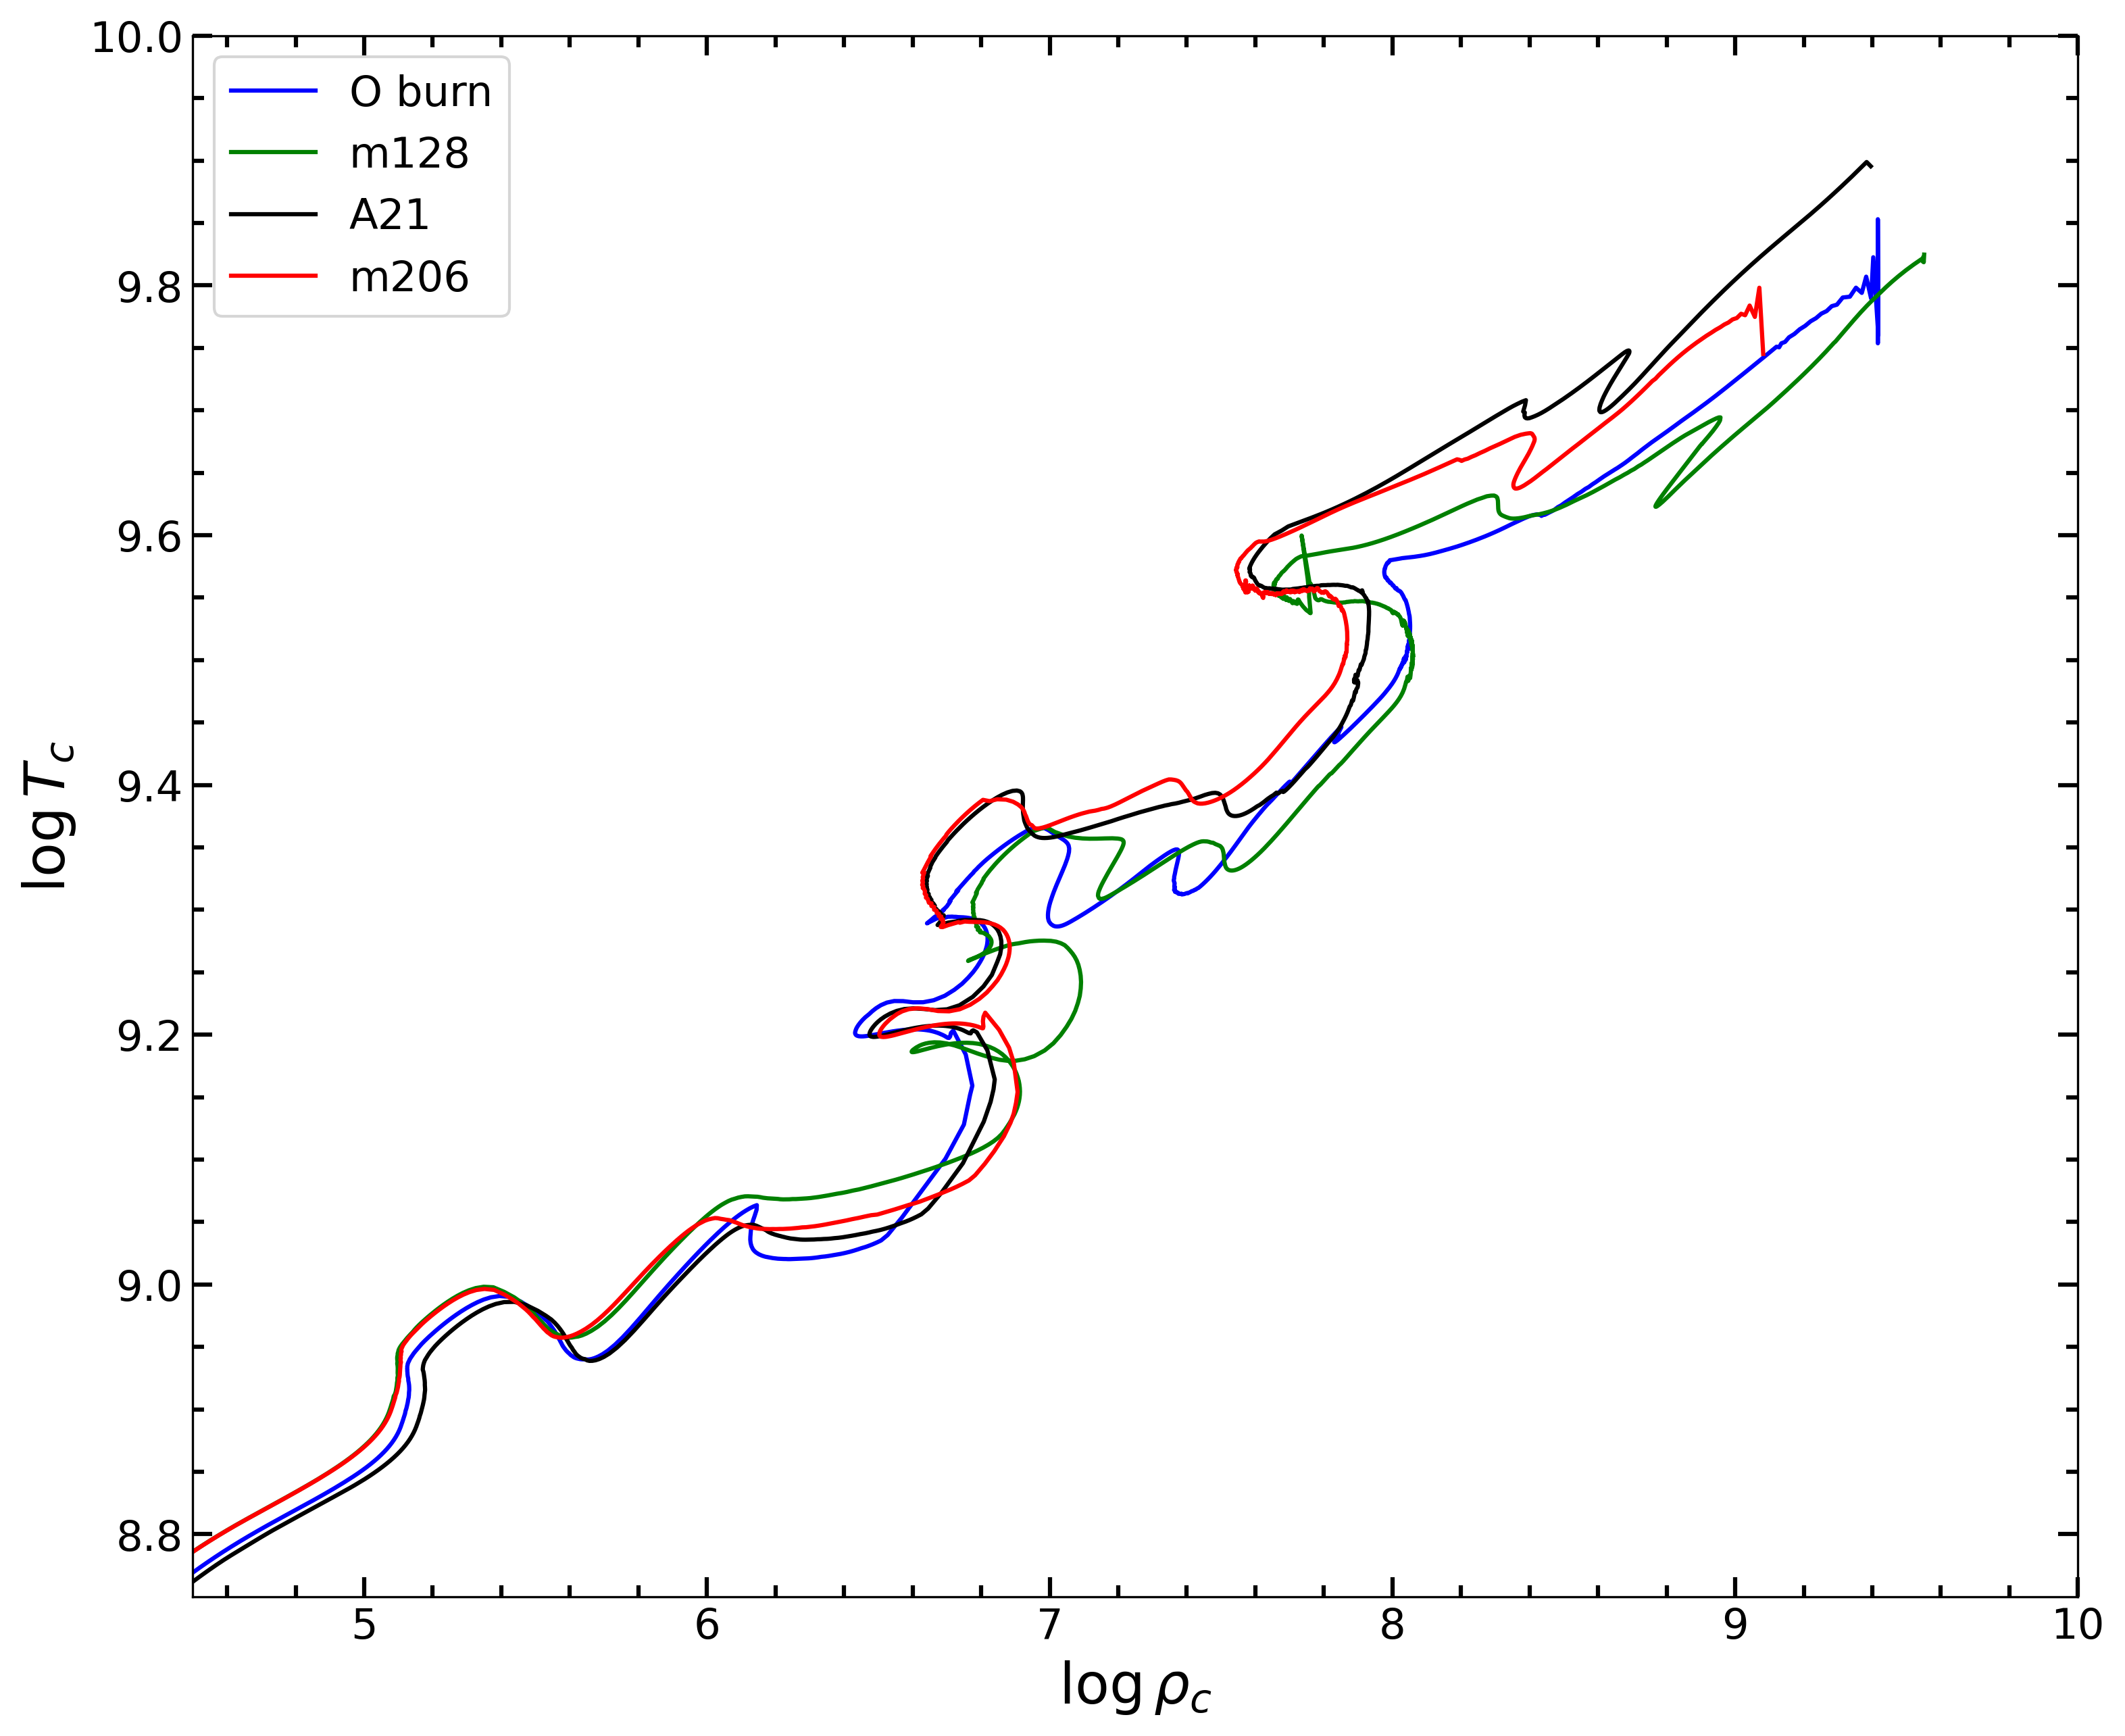
\includegraphics[width=\textwidth]{Varying Nuclear Networks/tcrhoc_ZOOM.png}
    \captionof{figure}{A detailed look in the \( T_c \) - \( \rho_c \) plane during advance burning stages}
    \label{fig:tcrhoczoom}
\end{minipage}

\vspace{1em}
\begin{center}
    \includegraphics[width=0.825\textwidth]{Varying Nuclear Networks/HRD.png}
\end{center}
\captionof{figure}{HR Diagram for the 20M\(_\odot \) models with different nuclear networks; the coloured dots on the path respectively refer to main sequence phase / H ignition (Pink), core H exhaustion / He ignition (Green), core He exhaustion / C ignition (Red).}
\label{fig:HRD}

\vspace{1em}
\noindent
Figure~\ref{fig:HRD} shows the evolutionary change of the star’s core properties, and Figure~\ref{fig:NucKips} illustrates the evolutionary tracks of the model in the HRD. Figures~\ref{fig:YevTc} and \ref{fig:NucKips} depicts the evolution of Y$_e$ against T$_c$ and the Kippenhahn plots for the different nuclear networks, representing the evolution of the convective regions and the location of the burning shells in mass in the star's interior. Each of these burning shells is discussed in brief in latter sections.

\begin{table}[h]
    \centering
    \caption{Physical properties of evolutionary models with different nuclear networks}
    \begin{tabular}{lcccccccc}
        \toprule
        Stage & \multicolumn{1}{c}{Star Age} & \multicolumn{1}{c}{$\log L / L_{\odot}$} & \multicolumn{1}{c}{$\log T_{\text{eff}}$} & \multicolumn{1}{c}{$T_c^a$} & \multicolumn{1}{c}{$\rho_c^b$} & \multicolumn{1}{c}{$M_{\alpha}^c$} & \multicolumn{1}{c}{$M_{C/O}^d$} & \multicolumn{1}{c}{$M_{ONe}^e$} \\
        & (yr) &  & (K) & ($10^7$K) & (g/cm$^3$) & ($M_{\odot}$) & ($M_{\odot}$) & ($M_{\odot}$) \\
        \midrule
        \multicolumn{9}{c}{\textbf{20M$_\odot$, f=0.05, A21.net}} \\
        \midrule
        \textbf{H$_{ignition}$} & $8.356 \times 10^4$ & 4.618 & 4.544 & 3.633  & 5.078 & 0.000 & 0.000 & 0.000  \\
        \textbf{H$_{exhaustion}$} & $9.214 \times 10^6$ & 5.032 & 4.387 & 5.663  & 15.34 & 6.422 & 0.000 & 0.000  \\
        \textbf{He$_{ignition}$} & $9.239 \times 10^6$ & 5.120 & 4.023 & 16.82  & 700.8 & 6.003 & 0.000 & 0.000  \\
        \textbf{He$_{exhaustion}$} & $1.004 \times 10^7$ & 5.127 & 3.507 & 30.48  & 2948 & 6.897 & 4.865 & 0.000  \\
        \textbf{C$_{ignition}$} & $1.006 \times 10^7$  & 5.240 & 3.496 & 60.16  & $3.892 \times 10^4$ & 6.907 & 4.865 & 0.000  \\
        \textbf{C$_{exhaustion}$} & $1.006 \times 10^7$  & 5.270 & 3.494 & 108.2  & $1.085 \times 10^6$ & 6.907  & 4.866  & 1.446  \\
        \textbf{O$_{ignition}$} & $1.006 \times 10^7$  & 5.264 & 3.494 & 166.1  & $5.018 \times 10^6$ & 6.906  & 4.866  & 4.224  \\
        \textbf{O$_{exhaustion}$} & $1.006 \times 10^7$  & 5.265 & 3.495 & 238.3  & $1.779 \times 10^7$ & 6.906  & 4.865  & 4.358  \\
	\midrule
	\multicolumn{9}{c}{\textbf{20M$_\odot$, f=0.05, OB.net}} \\
	\midrule
        \textbf{H$_{ignition}$} & $8.562 \times 10^4$  & 4.618 & 4.544 & 3.633  & 5.080 & 0.000  & 0.000  & 0.000  \\
        \textbf{H$_{exhaustion}$} & $9.158 \times 10^6$  & 5.052 & 4.402 & 5.684  & 15.13 & 6.533  & 0.000  & 0.000  \\
        \textbf{He$_{ignition}$} & $9.180 \times 10^6$  & 4.848 & 3.590 & 17.17  & 726.2    & 6.628  & 0.000  & 0.000  \\
        \textbf{He$_{exhaustion}$} & $9.896 \times 10^6$  & 5.094 & 3.518 & 30.19 & 2738  & 7.234  & 5.184  & 0.000  \\
        \textbf{C$_{ignition}$} & $9.910 \times 10^6$  & 5.301 & 3.499 & 82.69  & $1.353 \times 10^5$    & 7.235  & 5.185  & 0.000  \\
        \textbf{C$_{exhaustion}$} & $9.911 \times 10^6$  & 5.298 & 3.499 & 110.0  & $1.077 \times 10^6$    & 7.235  & 5.185  & 1.533  \\
        \textbf{O$_{ignition}$} & $9.911 \times 10^6$  & 5.293 & 3.499 & 168.3  & $4.273 \times 10^6$    & 7.235  & 5.185  & 4.368  \\
        \textbf{O$_{exhaustion}$} & $9.911 \times 10^6$  & 5.294 & 3.499 & 231.2  & $3.753 \times 10^7$ & 7.235  & 5.185  & 4.706  \\
        \midrule
        \multicolumn{9}{c}{\textbf{20M$_\odot$, f=0.05, M128.net}} \\
        \midrule
	\textbf{H$_{ignition}$} & $8.707 \times 10^4$  & 4.623 & 4.545 & 3.639  & 5.075  & 0.000  & 0.000  & 0.000  \\
        \textbf{H$_{exhaustion}$} & $9.456 \times 10^6$  & 5.101 & 4.361 & 5.712  & 14.71 & 7.532  & 0.000  & 0.000  \\
        \textbf{He$_{ignition}$} & $9.477 \times 10^6$  & 5.230 & 3.507 & 17.40  & 638.0 & 7.555  & 0.000  & 0.000  \\
        \textbf{He$_{exhaustion}$} & $1.012 \times 10^7$  & 5.207 & 3.510 & 30.60 & 2525 & 8.194  & 6.067  & 0.000  \\
        \textbf{C$_{ignition}$} & $1.014 \times 10^7$  & 5.382 & 3.494 & 86.07  & $1.252 \times 10^5$ & 8.200  & 6.068  & 0.000  \\
        \textbf{C$_{exhaustion}$} & $1.014 \times 10^7$  & 5.379 & 3.494 & 111.8  & $9.390 \times 10^5$ & 8.200  & 6.068  & 1.685  \\
        \textbf{O$_{ignition}$} & $1.014 \times 10^7$  & 5.376 & 3.494 & 154.0  & $9.668 \times 10^6$ & 8.200  & 6.068  & 1.785  \\
        \textbf{O$_{exhaustion}$} & $1.014 \times 10^7$  & 5.378 & 3.495 & 226.1  & $2.727 \times 10^7$ & 8.200  & 6.066  & 2.612  \\
        \midrule
        \multicolumn{9}{c}{\textbf{20M$_\odot$, f=0.05, M206.net}} \\
        \midrule
        \textbf{H$_{ignition}$} & $8.707 \times 10^4$  & 4.623 & 4.545 & 3.639  & 5.075 & 0.000  & 0.000  & 0.000  \\
        \textbf{H$_{exhaustion}$} & $9.456 \times 10^6$  & 5.101 & 4.361 & 5.712  & 14.71 & 7.532  & 0.000  & 0.000  \\
        \textbf{He$_{ignition}$} & $9.477 \times 10^6$  & 5.230 & 3.507 & 17.40  & 638.0 & 7.555  & 0.000  & 0.000  \\
        \textbf{He$_{exhaustion}$} & $1.012 \times 10^7$  & 5.207 & 3.510 & 30.60 & 2525 & 8.194  & 6.067  & 0.000  \\
        \textbf{C$_{ignition}$} & $1.014 \times 10^7$  & 5.381 & 3.495 & 87.00  & $1.275 \times 10^5$  & 8.190  & 6.073  & 0.000  \\
        \textbf{C$_{exhaustion}$} & $1.014 \times 10^7$  & 5.379 & 3.494 & 111.8  & $9.390 \times 10^5$  & 8.200  & 6.068  & 1.685  \\
        \textbf{O$_{ignition}$} & $1.014 \times 10^7$  & 5.376 & 3.494 & 154.0  & $9.668 \times 10^6$ & 8.200  & 6.068  & 1.785  \\
        \textbf{O$_{exhaustion}$} & $1.014 \times 10^7$  & 5.378 & 3.495 & 226.1 & $2.727 \times 10^7$ & 8.200  & 6.066  & 2.612  \\        	\bottomrule
    \end{tabular}
    \vspace{0.5em} \\
    \textbf{Note:} Superscripts a, b, c, d, e represent core temperature, core density, He, C/O and O/Ne core masses respectively.
    \label{tab:stellar_stages}
\end{table}

\begin{figure}[h!]
	\centering
	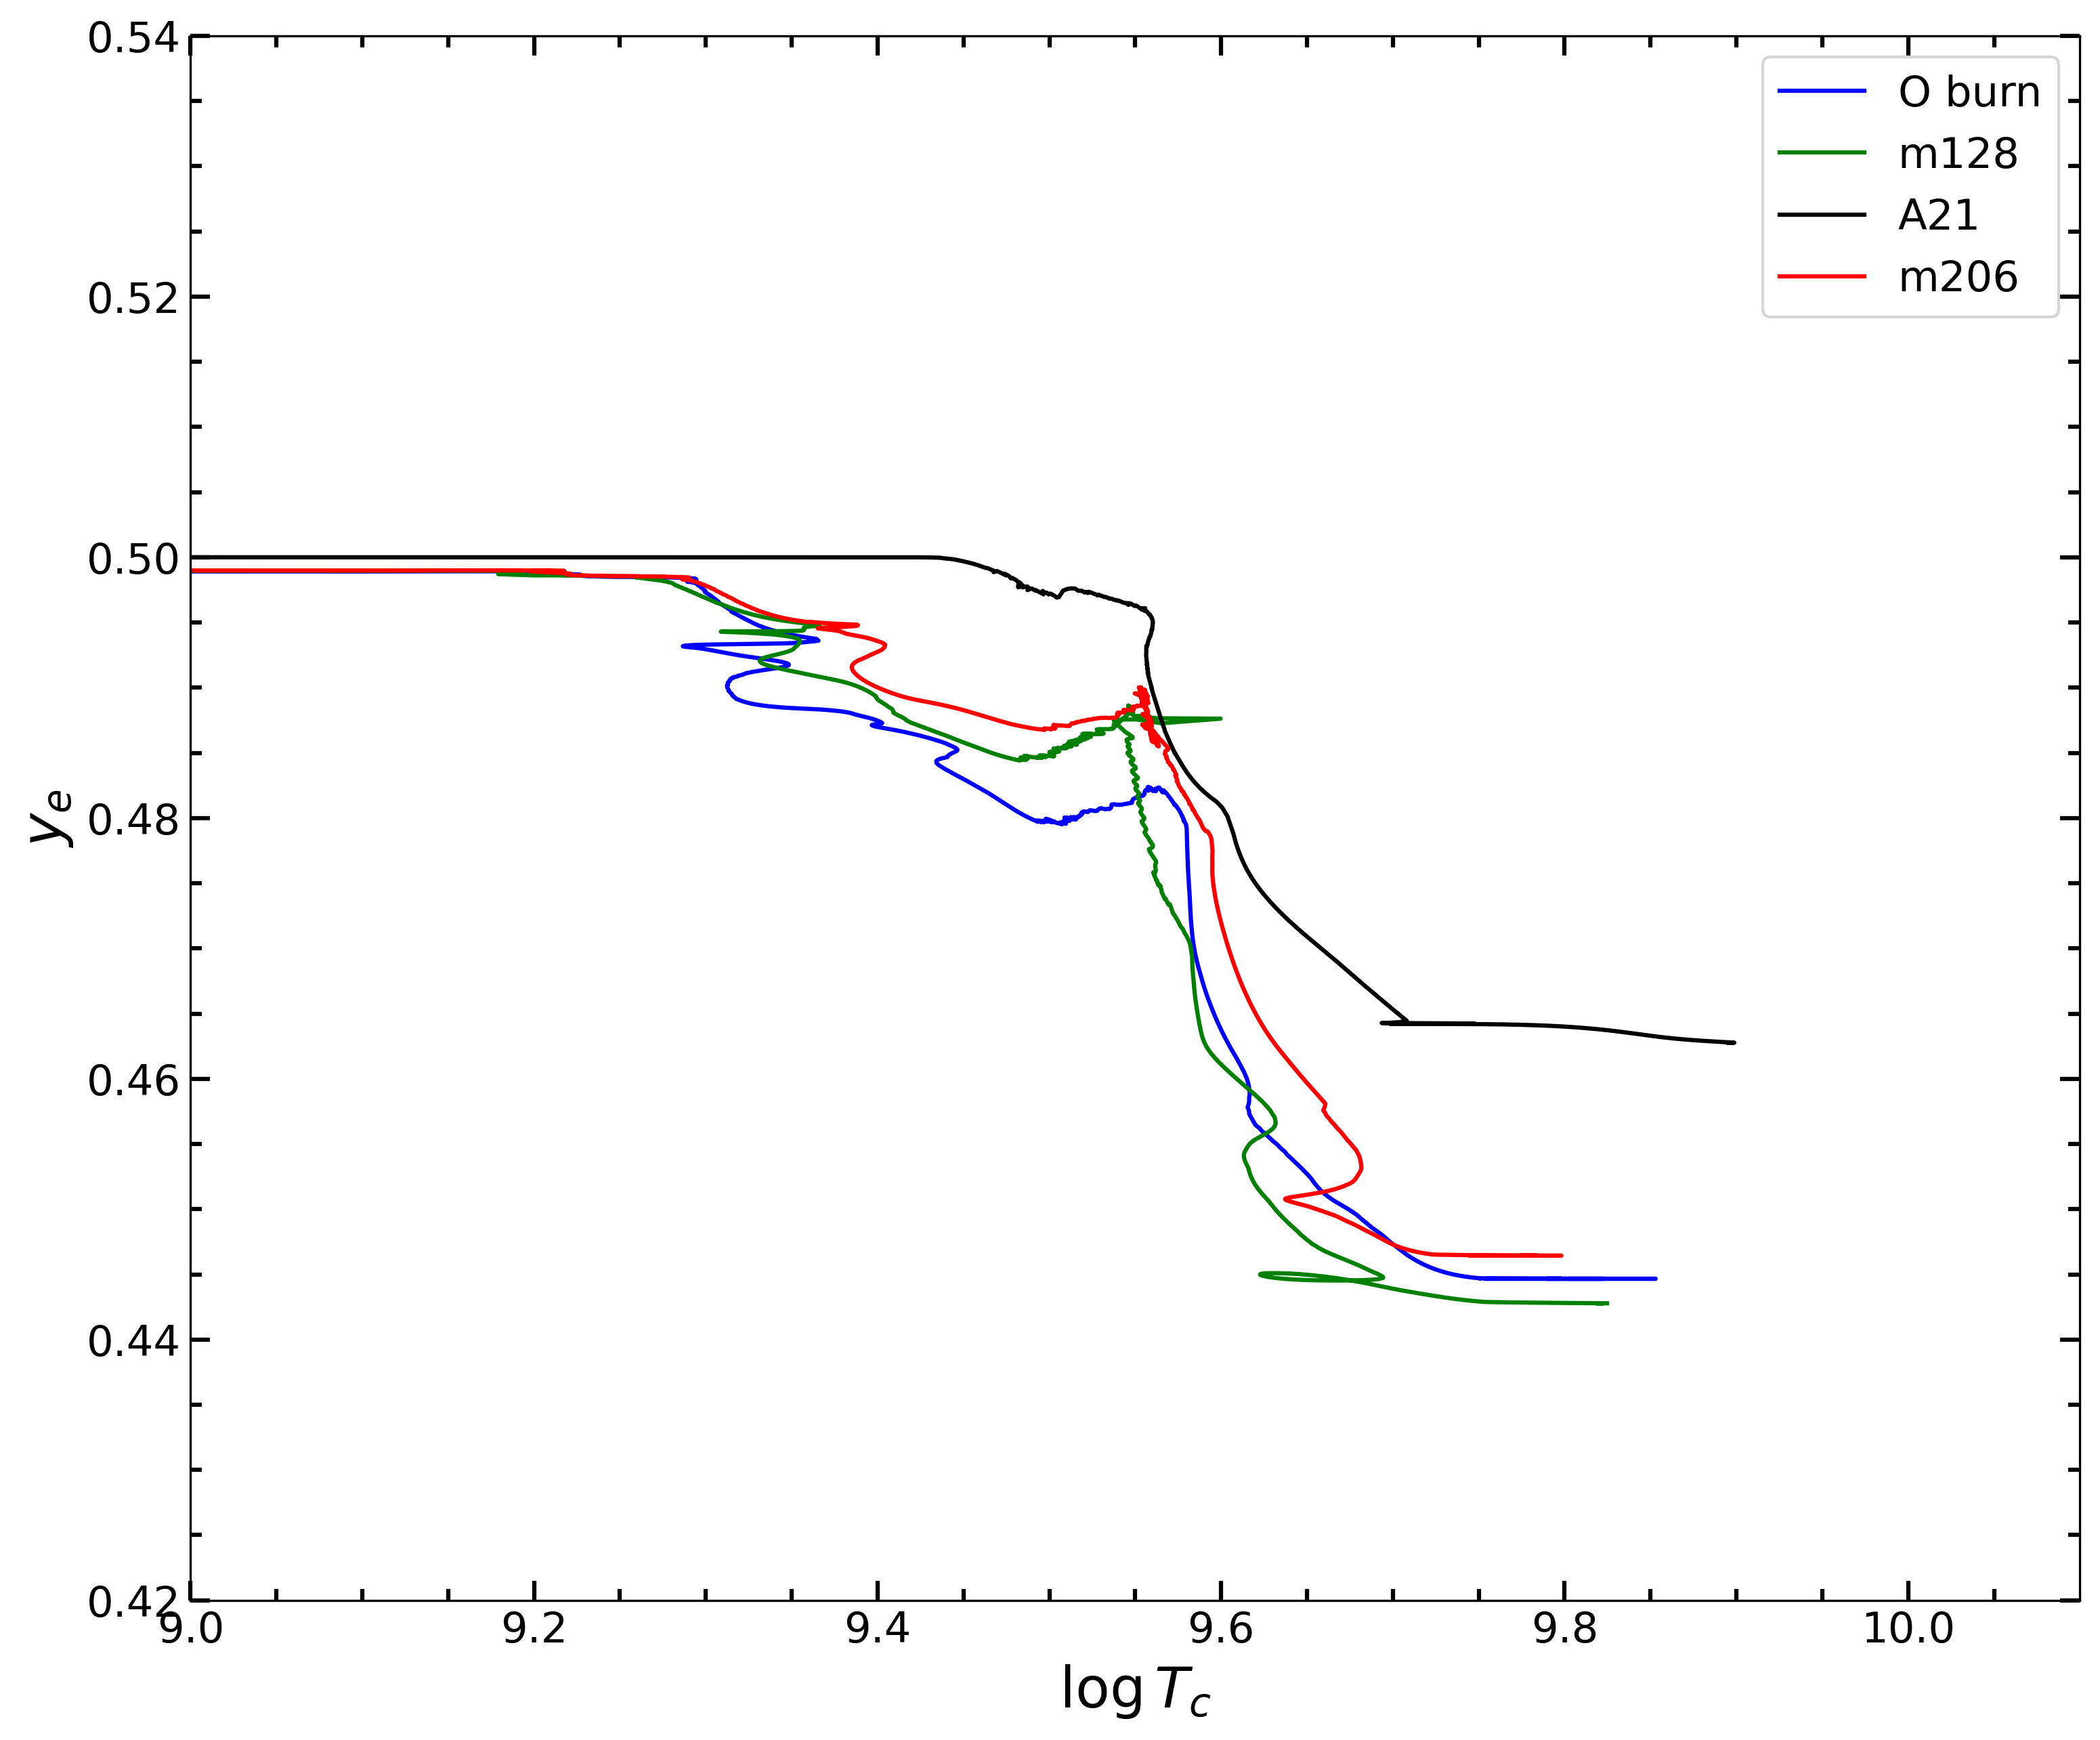
\includegraphics[width=0.51\textwidth]{Varying Nuclear Networks/yevtczoom.png}
	\captionof{figure}{Evolution of Ye vs Tc for different nuclear networks}
\label{fig:YevTc}
\end{figure}
\vspace{-1em}

\begin{figure}[h!]
    \centering
    \begin{subfigure}{0.49\textwidth}
        \centering
        \text{A21 Network} \\
        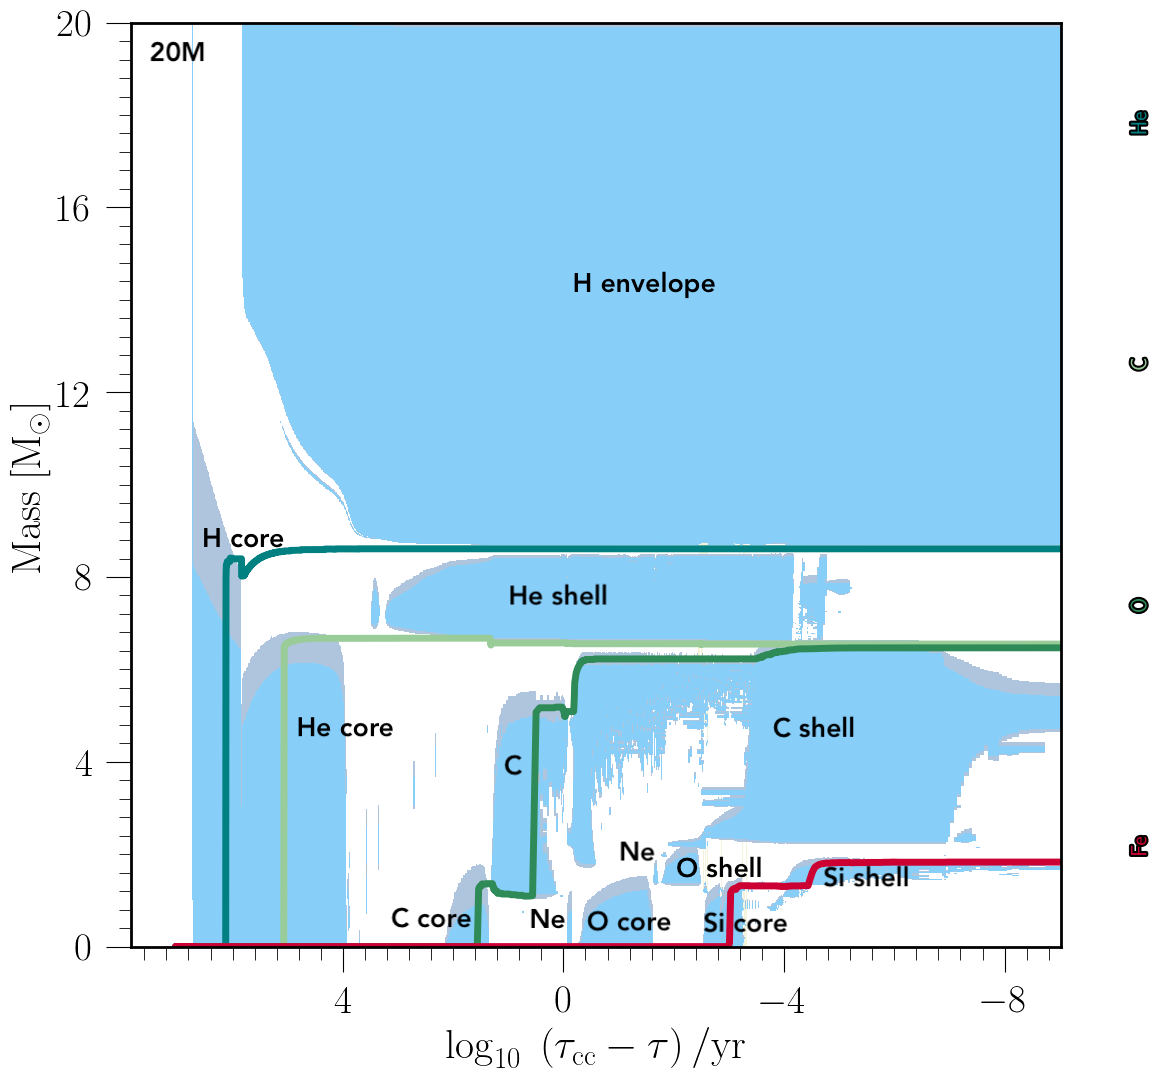
\includegraphics[width=\textwidth]{Varying Nuclear Networks/A21_KipCC.png}
    \end{subfigure}
    \begin{subfigure}{0.49\textwidth}
        \centering
        \text{O Burn Network} \\
        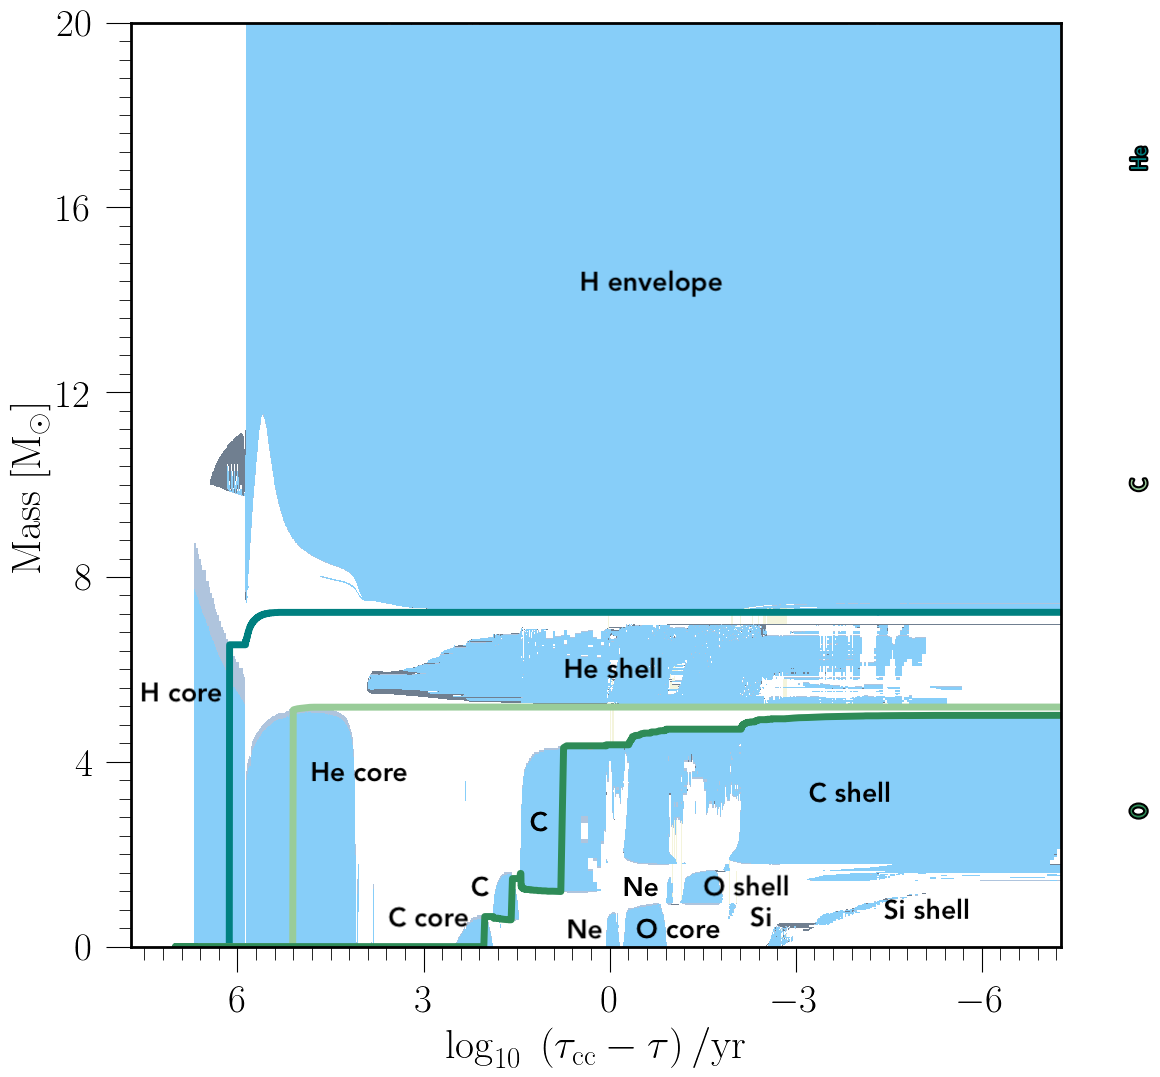
\includegraphics[width=\textwidth]{Varying Nuclear Networks/Ob_KipCC.png}
    \end{subfigure}
    \\[0.5em]
    \begin{subfigure}{0.49\textwidth}
        \centering
        \text{MESA 128 Network} \\
        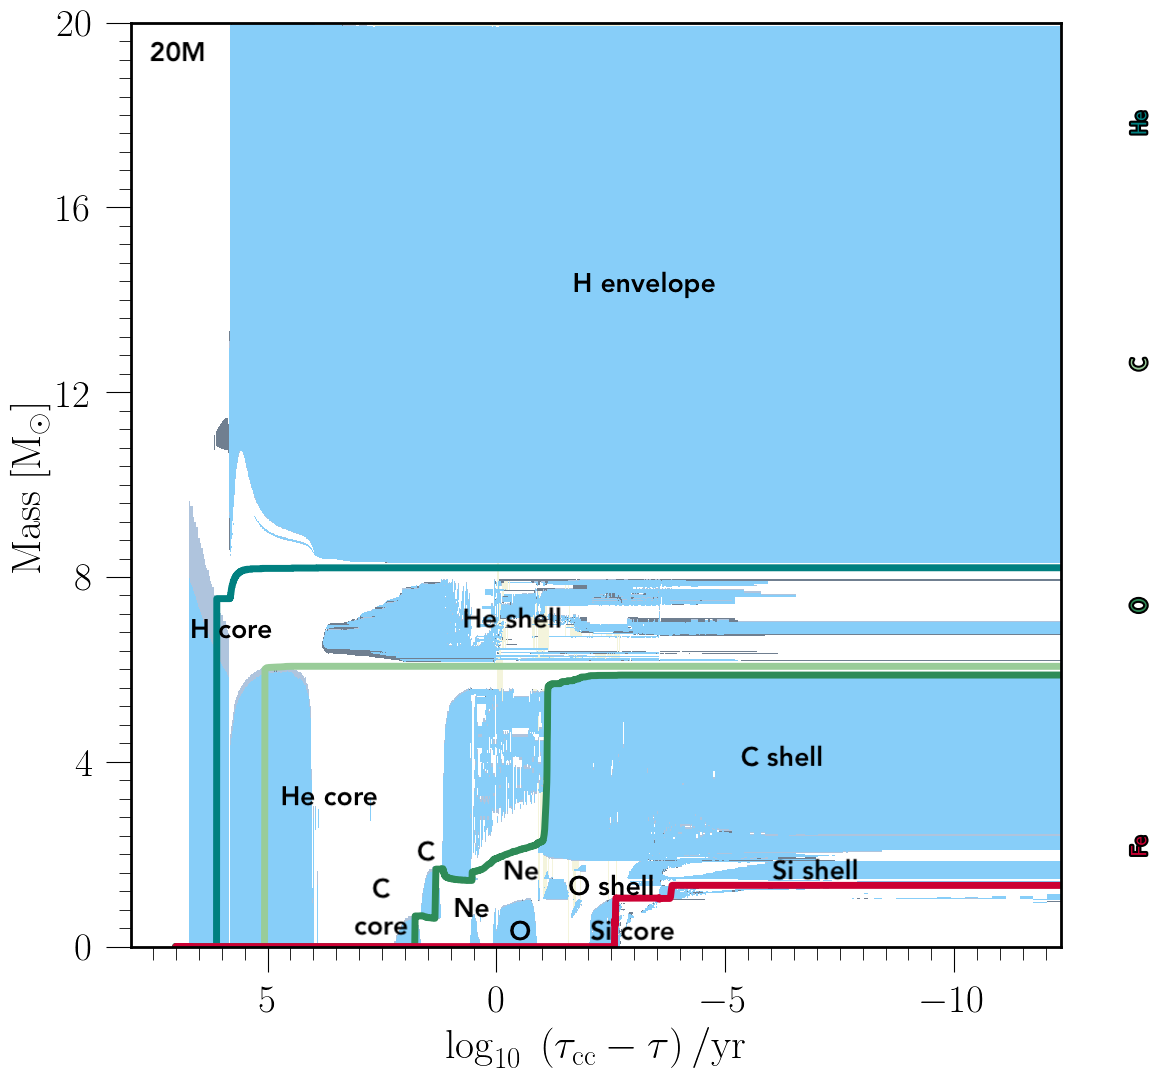
\includegraphics[width=\textwidth]{Varying Nuclear Networks/M128_KipCC.png}
    \end{subfigure}
    \begin{subfigure}{0.49\textwidth}
        \centering
        \text{MESA 206 Network} \\
        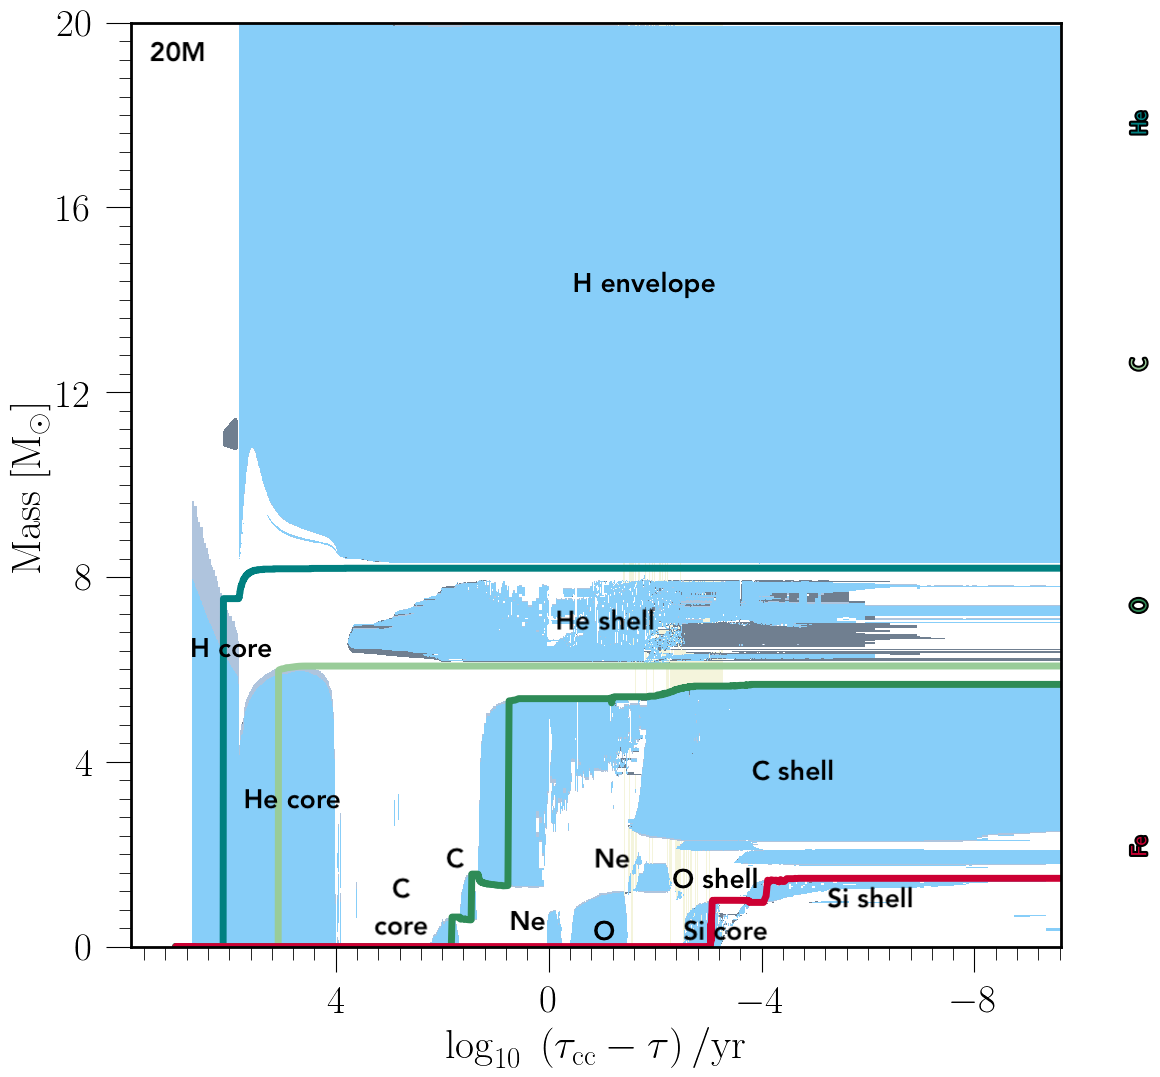
\includegraphics[width=\textwidth]{Varying Nuclear Networks/M206_KipCC.png}
    \end{subfigure}
    \caption{Kippenhahn plots for the 20M\(_\odot \) models with different nuclear networks.}
    \label{fig:NucKips}
\end{figure}

\clearpage
\subsection{Metallicity and Mass}
This section showcases the evolution of massive stars models with three distinct initial masses: 15, 20, and 25 M$_\odot$. These models are computed at seven different metallicities: solar metallicity, Z$_\odot$ ($\approx$ 0.0142), as well as lower metallicities of $10^{-3}$, $10^{-4}$, $10^{-5}$, $10^{-6}$, $10^{-7}$, and finally a zero-metallicity case representative of Population III stars. This broad metallicity range enables us to assess the influence of chemical composition on stellar structure and evolution—from metal-rich environments to nearly primordial conditions.

\vspace{1em}
\noindent
The physical properties of these 21 models—each corresponding to a specific mass and metallicity combination at key burning stages—are summarized in Tables~\ref{tab:HIEVMZ}, \ref{tab:HeIEVMZ}, \ref{tab:CIEVMZ}, and \ref{tab:OIEVMZ}. Furthermore, Figures~\ref{fig:15M-5CBM}, \ref{fig:20M-5CBM}, and \ref{fig:25M-5CBM} display the evolution of these models in both the HRD and the \(T_c\)-\(\rho_c\) plane, they illustrate how variations in mass and metallicity shape the evolutionary trajectories of stars, highlighting systematic trends such as shifts in luminosity and effective temperature during key phases of stellar evolution.

\subsection{Convective Boundary Mixing}
This section examines the impact of CBM on the evolution of massive stars by comparing models computed with three different overshoot parameters—corresponding to CBM rates of 5\%, 2\%, and 0.5\%—for stars with initial masses of 15, 20, and 25 M$_\odot$. CBM describes the process by which turbulent motions in convective zones penetrate into the adjacent radiative regions, thereby facilitating additional mixing beyond the classical convective boundaries defined by the Schwarzschild (or Ledoux) criteria.

\vspace{1em}
\noindent
By allowing convective eddies to overshoot into the stable layers, CBM can effectively enlarge the convective core, alter the chemical gradients, and extend the duration of core burning phases. These effects have significant consequences for the star's evolutionary trajectory, influencing both the position of the star in the HRD and the \(T_c\)-\(\rho_c\)) structure.

\vspace{1em}
\noindent
Figures~\ref{fig:15M_CBM_Comparison}, \ref{fig:20M_CBM_Comparison}, and \ref{fig:25M_CBM_Comparison} illustrate the evolutionary tracks in both the HRD and the \(T_c\)-\(\rho_c\) plane for the 15, 20, and 25 M$_\odot$ models with three different CBM rates respectively. These figures vividly demonstrate that higher CBM rates lead to more extended convective cores, longer main-sequence lifetimes, and systematic shifts in the evolutionary paths, while lower CBM rates result in more compact cores and alternate evolutionary characteristics. 

\begin{table}[h!]
    \centering
    \caption{Properties of models with varying mass and metallicity during H burning stage}
    \resizebox{\textwidth}{!}{
    \begin{tabular}{lcccccccc}
        \toprule
        Z & M($M_\odot$) & \multicolumn{1}{c}{Star Age (yr)} & \multicolumn{1}{c}{$\log (L / L_{\odot})$} & \multicolumn{1}{c}{$\log T_{\text{eff}}$ (K)} & \multicolumn{1}{c}{$T_c^a$ ($10^7$ K)} & \multicolumn{1}{c}{$\rho_c^b$ (g cm$^{-3}$)} & \multicolumn{1}{c}{$M_{cc}^e$ ($M_{\odot}$)} \\
        \midrule
        \multicolumn{8}{c}{\textbf{ ZAMS ( Hydrogen ignition )}} \\
        \midrule
        Z$_\odot$ & 15 & $1.524 \times 10^5$  & 4.270 & 4.492 & 3.463 & 6.554  & 5.758  \\
                  & 20 & $9.167 \times 10^4$  & 4.618 & 4.544 & 3.633 & 5.078  & 8.887  \\
                  & 25 & $6.528 \times 10^4$  & 4.869 & 4.580 & 3.758 & 4.241  & 12.44  \\
        $10^{-3}$ & 15 & $1.441 \times 10^5$  & 4.316 & 4.551 & 3.928 & 9.697  & 6.187  \\
                  & 20 & $8.719 \times 10^4$  & 4.650 & 4.597 & 4.117 & 7.492  & 9.419  \\
                  & 25 & $6.604 \times 10^4$  & 4.893 & 4.630 & 4.258 & 6.254  & 13.04  \\
        $10^{-4}$ & 15 & $1.419 \times 10^5$  & 4.325 & 4.584 & 4.403 & 13.68  & 6.255  \\
                  & 20 & $8.619 \times 10^4$  & 4.657 & 4.629 & 4.626 & 10.65  & 9.457  \\
                  & 25 & $6.778 \times 10^4$  & 4.899 & 4.662 & 4.792 & 8.928  & 13.07  \\
        $10^{-5}$ & 15 & $1.496 \times 10^5$  & 4.330 & 4.616 & 5.051 & 20.70  & 6.246  \\
                  & 20 & $9.190 \times 10^4$  & 4.661 & 4.662 & 5.320 & 16.23  & 9.445  \\
                  & 25 & $6.951 \times 10^4$  & 4.903 & 4.694 & 5.520 & 13.67  & 13.04  \\
        $10^{-6}$ & 15 & $1.476 \times 10^5$  & 4.335 & 4.649 & 5.824 & 31.80  & 6.213  \\
                  & 20 & $9.513 \times 10^4$  & 4.666 & 4.695 & 6.153 & 25.15  & 9.422  \\
                  & 25 & $7.345 \times 10^4$  & 4.907 & 4.728 & 6.397 & 21.30  & 13.01  \\
        $10^{-7}$ & 15 & $1.499 \times 10^5$  & 4.340 & 4.682 & 6.742 & 49.44  & 6.165  \\
                  & 20 & $9.573 \times 10^4$  & 4.671 & 4.729 & 7.152 & 39.57  & 9.357  \\
                  & 25 & $7.438 \times 10^4$  & 4.912 & 4.762 & 7.455 & 33.77  & 12.93  \\
        $0$ & 15 & $1.001 \times 10^5$ & 4.458 & 4.757 & 9.033 & 137.7 & 0.000 \\
            & 20 & $7.807 \times 10^4$ & 4.780 & 4.828 & 10.85 & 151.6 & 1.325 \\
            & 25 & $7.643 \times 10^4$ & 4.949 & 4.863 & 11.60 & 128.4 & 12.03 \\
        \midrule
        \multicolumn{8}{c}{\textbf{ Hydrogen Exhaustion }} \\
        \midrule
        Z$_\odot$ & 15 & $1.581 \times 10^7$  & 4.913 & 4.283 & 5.571 & 17.01 & 4.452  \\
          & 20 & $1.005 \times 10^7$  & 5.149 & 4.304 & 5.753 & 14.42 & 6.364  \\
          & 25 & $7.795 \times 10^6$  & 5.365 & 4.276 & 5.950 & 12.59 & 8.955  \\
	$10^{-3}$ & 15 & $1.485 \times 10^7$  & 4.943 & 4.421 & 6.631 & 28.42 & 4.586  \\
          & 20 & $9.805 \times 10^6$  & 5.185 & 4.440 & 6.872 & 24.13 & 6.622  \\
          & 25 & $7.694 \times 10^6$  & 5.394 & 4.441 & 7.108 & 21.18 & 9.235  \\
	$10^{-4}$ & 15 & $1.451 \times 10^7$  & 4.945 & 4.475 & 7.754 & 45.87 & 4.521  \\
          & 20 & $9.696 \times 10^6$  & 5.192 & 4.493 & 8.050 & 38.83 & 6.608  \\
          & 25 & $7.625 \times 10^6$  & 5.400 & 4.497 & 8.333 & 34.17 & 9.202  \\
	$10^{-5}$ & 15 & $1.429 \times 10^7$  & 4.950 & 4.513 & 9.107 & 74.64 & 4.469  \\
          & 20 & $9.578 \times 10^6$  & 5.197 & 4.531 & 9.521 & 64.61 & 6.519  \\
          & 25 & $7.540 \times 10^6$  & 5.404 & 4.536 & 9.831 & 56.41 & 9.100  \\
	$10^{-6}$ & 15 & $1.398 \times 10^7$  & 4.959 & 4.549 & 10.82 & 125.6 & 4.409  \\
          & 20 & $9.401 \times 10^6$  & 5.200 & 4.567 & 11.25 & 107.4 & 6.426  \\
          & 25 & $7.423 \times 10^6$  & 5.407 & 4.571 & 11.63 & 94.03 & 8.984  \\
	$10^{-7}$ & 15 & $1.343 \times 10^7$  & 4.964 & 4.581 & 12.47 & 192.1 & 4.424  \\
          & 20 & $9.111 \times 10^6$  & 5.199 & 4.598 & 12.82 & 159.5 & 6.389  \\
          & 25 & $7.231 \times 10^6$  & 5.405 & 4.600 & 13.08 & 134.2 & 8.926  \\
	$0$       & 15 & $1.033 \times 10^7$  & 4.966 & 4.585 & 12.58 & 195.9 & 4.468  \\
          & 20 & $7.718 \times 10^6$  & 5.192 & 4.607 & 12.87 & 162.3 & 6.316  \\
          & 25 & $6.427 \times 10^6$  & 5.399 & 4.608 & 13.10 & 135.5 & 8.829  \\
         \bottomrule    
        \end{tabular}}
    \label{tab:HIEVMZ}
\end{table}

\clearpage
{
\renewcommand{\arraystretch}{0.96}
\begin{table}[h!]
    \centering
    \caption{Properties of models with varying mass and metallicity during He burning stage.}
    \resizebox{\textwidth}{!}{
    \begin{tabular}{lcccccccccc}
        \toprule
        Z & M & Star Age & $\log (L / L_{\odot})$ & $\log T_{\text{eff}}$ & $T_c^a$ & $\rho_c^b$ & $M_{\alpha}^c$ & $M_{C/O}^d$ & $M_{cc}^e$ \\
    & ($M_{\odot}$) & (yr) &  & (K) & ($10^7$ K) & (g cm$^{-3}$) & ($M_{\odot}$) & ($M_{\odot}$) & ($M_{\odot}$) \\
        \midrule
        \multicolumn{10}{c}{\textbf{ Helium Ignition }} \\
        \midrule
        $Z_{\odot}$ & 15 & $1.584 \times 10^7$  & 5.127 & 3.503 & 16.79 & 715 & 6.104  & 0.000  & 2.772  \\
                    & 20 & $1.007 \times 10^7$  & 5.234 & 3.766 & 17.21 & 547 & 8.020  & 0.000  & 4.420  \\
                    & 25 & $7.812 \times 10^6$  & 5.435 & 3.642 & 17.57 & 435 & 10.61  & 0.000  & 6.551  \\
        $10^{-3}$   & 15 & $1.487 \times 10^7$  & 5.015 & 3.764 & 17.47 & 797 & 6.271  & 0.000  & 2.381  \\
                    & 20 & $9.822 \times 10^6$  & 5.256 & 4.192 & 18.09 & 610 & 8.702  & 0.000  & 3.670  \\
                    & 25 & $7.708 \times 10^6$  & 5.449 & 4.234 & 18.64 & 492 & 11.78  & 0.000  & 5.729  \\
        $10^{-4}$   & 15 & $1.453 \times 10^7$  & 5.022 & 4.316 & 17.53 & 785 & 6.227  & 0.000  & 2.240  \\
                    & 20 & $9.712 \times 10^6$  & 5.278 & 4.429 & 18.14 & 606 & 8.214  & 0.000  & 3.707  \\
                    & 25 & $7.638 \times 10^6$  & 5.476 & 4.449 & 18.67 & 492 & 11.04  & 0.000  & 5.750  \\
        $10^{-5}$   & 15 & $1.431 \times 10^7$  & 4.984 & 4.443 & 17.54 & 741 & 6.215  & 0.000  & 2.240  \\
                    & 20 & $9.592 \times 10^6$  & 5.217 & 4.503 & 18.18 & 566 & 8.718  & 0.000  & 3.826  \\
                    & 25 & $7.551 \times 10^6$  & 5.425 & 4.531 & 18.71 & 458 & 11.75  & 0.000  & 6.048  \\
        $10^{-6}$   & 15 & $1.399 \times 10^7$  & 4.981 & 4.546 & 17.60 & 679 & 6.227  & 0.000  & 2.526  \\
                    & 20 & $9.413 \times 10^6$  & 5.224 & 4.581 & 18.27 & 529 & 8.583  & 0.000  & 4.385  \\
                    & 25 & $7.432 \times 10^6$  & 5.433 & 4.591 & 18.87 & 440 & 11.55  & 0.000  & 6.953  \\
        $10^{-7}$   & 15 & $1.344 \times 10^7$  & 4.999 & 4.596 & 17.89 & 635 & 6.125  & 0.000  & 3.206  \\
                    & 20 & $9.121 \times 10^6$  & 5.228 & 4.616 & 18.52 & 520 & 8.557  & 0.000  & 5.145  \\
                    & 25 & $7.239 \times 10^6$  & 5.430 & 4.619 & 19.05 & 439 & 11.41  & 0.000  & 7.596  \\
        $0$         & 15 & $1.034 \times 10^7$  & 5.008 & 4.604 & 18.05 & 631 & 6.199  & 0.000  & 3.505  \\
                    & 20 & $7.727 \times 10^6$  & 5.223 & 4.627 & 18.57 & 523 & 8.407  & 0.000  & 5.199  \\
                    & 25 & $6.436 \times 10^6$  & 5.424 & 4.628 & 19.07 & 441 & 11.37  & 0.000  & 7.612  \\
        \midrule
	\multicolumn{10}{c}{\textbf{ Helium Exhaustion }} \\
	\midrule
	$Z_{\odot}$ & 15 & $1.663 \times 10^7$  & 5.156 & 3.502 & 30.32 & 2779 & 7.116 & 5.315 & 4.421  \\
                    & 20 & $1.074 \times 10^7$  & 5.271 & 3.510 & 31.01 & 2491 & 8.609 & 6.674 & 5.696  \\
                    & 25 & $8.359 \times 10^6$  & 5.452 & 3.511 & 31.84 & 2140 & 11.24 & 9.147 & 8.005  \\
        $10^{-3}$   & 15 & $1.565 \times 10^7$  & 5.175 & 3.580 & 30.57 & 2741 & 7.341 & 5.596 & 4.625  \\
                    & 20 & $1.044 \times 10^7$  & 5.321 & 3.591 & 31.31 & 2348 & 9.454 & 7.503 & 6.466  \\
                    & 25 & $8.219 \times 10^6$  & 5.505 & 3.590 & 32.13 & 2025 & 12.38 & 10.24 & 9.047  \\
        $10^{-4}$   & 15 & $1.532 \times 10^7$  & 5.160 & 3.617 & 30.46 & 2741 & 7.208 & 5.479 & 4.552  \\
                    & 20 & $1.035 \times 10^7$  & 5.345 & 4.080 & 31.25 & 2409 & 9.039 & 7.109 & 6.090  \\
                    & 25 & $8.164 \times 10^6$  & 5.527 & 4.116 & 32.05 & 2088 & 11.72 & 9.529 & 8.376  \\
        $10^{-5}$   & 15 & $1.505 \times 10^7$  & 5.133 & 3.927 & 30.51 & 2751 & 7.110 & 5.500 & 4.493  \\
                    & 20 & $1.018 \times 10^7$  & 5.326 & 3.617 & 31.30 & 2296 & 9.472 & 7.725 & 6.573  \\
                    & 25 & $8.041 \times 10^6$  & 5.543 & 3.615 & 32.14 & 1988 & 12.43 & 10.49 & 9.188  \\
        $10^{-6}$   & 15 & $1.471 \times 10^7$  & 5.119 & 4.180 & 30.39 & 2757 & 6.856 & 5.384 & 4.343  \\
                    & 20 & $9.983 \times 10^6$  & 5.323 & 3.914 & 31.37 & 2336 & 9.190 & 7.566 & 6.346  \\
                    & 25 & $7.910 \times 10^6$  & 5.534 & 3.616 & 32.04 & 1985 & 12.12 & 10.30 & 8.942  \\
        $10^{-7}$   & 15 & $1.412 \times 10^7$  & 5.106 & 4.299 & 30.28 & 2759 & 6.585 & 5.278 & 4.158  \\
                    & 20 & $9.668 \times 10^6$  & 5.316 & 4.123 & 31.08 & 2296 & 8.885 & 7.391 & 6.120  \\
                    & 25 & $7.702 \times 10^6$  & 5.522 & 3.616 & 32.07 & 2011 & 11.76 & 10.07 & 8.581  \\
        $0$         & 15 & $1.099 \times 10^7$  & 5.094 & 4.407 & 30.07 & 2687 & 6.304 & 5.260 & 4.091  \\
                    & 20 & $8.263 \times 10^6$  & 5.299 & 4.314 & 31.18 & 2338 & 8.510 & 7.256 & 5.926  \\
                    & 25 & $6.893 \times 10^6$  & 5.498 & 4.008 & 31.91 & 1988 & 11.41 & 9.927 & 8.460  \\
        \bottomrule    
        \end{tabular}}
    \label{tab:HeIEVMZ}
\end{table}
}

\clearpage
{
\renewcommand{\arraystretch}{1.075}
\begin{table}[h!]
    \centering
    \caption{Properties of models with varying mass and metallicity during C burning stage.}
    \resizebox{\textwidth}{!}{
    \begin{tabular}{lccccccccccc}
        \toprule
        $Z$ & $M_\odot$ & Star Age & $\log (L / L_{\odot})$ & $\log T_{\text{eff}}$ & $T_c^a$ & $\rho_c^b$ & $M_{\alpha}^c$ & $M_{C/O}^d$ & $M_{ONe}^e$ & $M_{cc}^f$ \\
    & ($M_{\odot}$) & (yr) &  & (K) & ($10^7$ K) & (g cm$^{-3}$) & ($M_{\odot}$) & ($M_{\odot}$) & ($M_{\odot}$) & ($M_{\odot}$) \\
        \midrule
        \multicolumn{11}{c}{\textbf{ Carbon Ignition }} \\
        \midrule
        $Z_{\odot}$ & 15 & $1.644 \times 10^7$  & 5.261 & 3.493 & 52.43 & 17780 & 7.122  & 5.315  & 0.000  & 0.000  \\
                    & 20 & $1.075 \times 10^7$  & 5.362 & 3.501 & 55.45 & 17420 & 8.611  & 6.674  & 0.000  & 0.000  \\
                    & 25 & $8.366 \times 10^6$  & 5.557 & 3.501 & 61.84 & 20130 & 11.24  & 9.147  & 0.000  & 0.000  \\
        $10^{-3}$ & 15 & $1.566 \times 10^7$  & 5.299 & 3.567 & 84.06 & $1.271 \times 10^5$ & 7.358  & 5.600  & 0.000  & 0.000  \\
                    & 20 & $1.045 \times 10^7$ & 5.450 & 3.572 & 97.57 & $4.047 \times 10^5$ & 9.454 & 7.457 & 0.800 & 0.000  \\
                    & 25 & $8.226 \times 10^6$  & 5.627 & 3.574 & 115.7 & $6.101 \times 10^5$ & 12.38  & 9.963  & 1.822  & 0.000  \\
        $10^{-4}$ & 15 & $1.533 \times 10^7$  & 5.275 & 3.607 & 84.04 & $1.319 \times 10^5$ & 7.212  & 5.483  & 0.000  & 0.224  \\
                    & 20 & $1.037 \times 10^7$  & 5.380 & 3.613 & 89.47 & $1.210 \times 10^5$ & 9.053  & 7.111  & 0.000  & 0.353 \\
                    & 25 & $8.172 \times 10^6$  & 5.501 & 3.620 & 101.8 & $3.322 \times 10^5$ & 11.67  & 9.333  & 1.024  & 0.000  \\
        $10^{-5}$ & 15 & $1.507 \times 10^7$  & 5.273 & 3.611 & 83.56 & $1.273 \times 10^5$ & 7.115  & 5.504  & 0.000  & 0.235 \\
                    & 20 & $1.019 \times 10^7$  & 5.496 & 3.609 & 99.78 & $4.306 \times 10^5$ & 9.493  & 7.676  & 1.007  & 0.000  \\
                    & 25 & $8.049 \times 10^6$  & 5.669 & 3.610 & 98.05 & $2.243 \times 10^5$ & 12.44  & 10.37  & 0.761  & 0.000  \\
        $10^{-6}$ & 15 & $1.473 \times 10^7$  & 5.254 & 3.612 & 82.85 & $1.270 \times 10^5$ & 6.881  & 5.390  & 0.000  & 0.224 \\
                    & 20 & $9.993 \times 10^6$  & 5.451 & 3.611 & 83.29 & $1.077 \times 10^5$ & 9.216  & 7.568  & 0.000  & 0.445 \\
                    & 25 & $7.918 \times 10^6$  & 5.595 & 3.612 & 93.00 & $1.440 \times 10^5$ & 12.14  & 10.26  & 0.221  & 0.000  \\
        $10^{-7}$ & 15 & $1.414 \times 10^7$  & 5.239 & 3.612 & 79.56 & $1.261 \times 10^5$ & 6.604  & 5.285  & 0.000  & 0.065 \\
                    & 20 & $9.679 \times 10^6$  & 5.425 & 3.611 & 8.276 & $1.056 \times 10^5$ & 8.874  & 7.394  & 0.000  & 0.002 \\
                    & 25 & $7.710 \times 10^6$  & 5.575 & 3.613 & 109.8 & $4.675 \times 10^5$ & 11.77  & 9.985  & 1.391  & 0.000  \\
        $Z=0$ & 15 & $1.100 \times 10^7$  & 5.013 & 3.656 & 82.81 & $41.225 \times 10^5$ & 6.313  & 5.268  & 0.000  & 0.289 \\
                    & 20 & $8.273 \times 10^6$  & 5.184 & 3.624 & 114.2 & $3.876 \times 10^5$ & 8.521  & 7.262  & 1.540  & 0.000  \\
                    & 25 & $6.902 \times 10^6$  & 5.568 & 3.613 & 110.8 & $4.780 \times 10^5$ & 11.59  & 9.931  & 1.463  & 0.000  \\
        \midrule
        \multicolumn{11}{c}{\textbf{ Carbon Exhaustion }} \\
        \midrule
        $Z_{\odot}$ & 15 & $1.664 \times 10^7$  & 5.289 & 3.490 & 107.3 & $6.274 \times 10^5$ & 7.125  & 5.319  & 1.210  & 0.000  \\
                    & 20 & $1.075 \times 10^7$  & 5.407 & 3.497 & 111.6 & $5.233 \times 10^5$ & 8.611  & 6.573  & 1.363  & 0.000  \\
                    & 25 & $8.367 \times 10^6$  & 5.558 & 3.501 & 109.8 & $6.182 \times 10^5$ & 11.24  & 8.924  & 1.249  & 0.000  \\
        $10^{-3}$   & 15 & $1.566 \times 10^7$  & 5.303 & 3.567 & 108.0 & $5.925 \times 10^5$ & 7.358  & 5.600  & 1.264  & 0.000  \\
                    & 20 & $1.045 \times 10^7$  & 5.450 & 3.572 & 115.8 & $8.937 \times 10^5$ & 9.454  & 7.431  & 2.283  & 0.000  \\
                    & 25 & $8.226 \times 10^6$  & 5.627 & 3.574 & 115.7 & $6.101 \times 10^5$ & 12.38  & 9.963  & 1.822  & 0.000  \\
        $10^{-4}$   & 15 & $1.533 \times 10^7$  & 5.277 & 3.607 & 107.4 & $6.036 \times 10^5$ & 7.212  & 5.484  & 1.224  & 0.000  \\
                    & 20 & $1.037 \times 10^7$  & 5.391 & 3.612 & 112.6 & $4.902 \times 10^5$ & 9.053  & 7.030  & 1.375  & 0.000  \\
                    & 25 & $8.172 \times 10^6$  & 5.501 & 3.620 & 114.2 & $6.334 \times 10^5$ & 11.67  & 9.290  & 1.543  & 0.000  \\
        $10^{-5}$   & 15 & $1.507 \times 10^7$  & 5.276 & 3.610 & 107.9 & $6.126 \times 10^5$ & 7.115  & 5.505  & 1.251  & 0.000  \\
                    & 20 & $1.019 \times 10^7$  & 5.495 & 3.609 & 114.5 & $9.300 \times 10^5$ & 9.528  & 7.655  & 2.606  & 0.000  \\
                    & 25 & $8.049 \times 10^6$  & 5.628 & 3.609 & 115.1 & $6.309 \times 10^5$ & 13.06  & 10.37  & 1.717  & 0.000  \\
        $10^{-6}$   & 15 & $1.473 \times 10^7$  & 5.236 & 3.612 & 106.4 & $7.067 \times 10^5$ & 7.350  & 5.390  & 1.244  & 0.000  \\
                    & 20 & $9.993 \times 10^6$  & 5.458 & 3.574 & 113.8 & $4.516 \times 10^5$ & 9.030  & 7.571  & 1.458  & 0.000  \\
                    & 25 & $7.918 \times 10^6$  & 5.472 & 3.546 & 110.9 & $6.655 \times 10^5$ & 10.46  & 10.26  & 1.357  & 0.000  \\
        $10^{-7}$   & 15 & $1.414 \times 10^7$  & 5.328 & 3.532 & 106.0 & $6.778 \times 10^5$ & 5.506  & 5.285  & 1.200  & 0.000  \\
                    & 20 & $9.679 \times 10^6$  & 5.393 & 3.500 & 111.0 & $5.416 \times 10^5$ & 7.318  & 7.318  & 1.351  & 0.000  \\
                    & 25 & $7.710 \times 10^6$  & 5.575 & 3.613 & 107.7 & $5.534 \times 10^5$ & 11.77  & 9.950  & 1.201  & 0.000  \\
        $0$         & 15 & $1.100 \times 10^7$  & 5.027 & 3.622 & 105.9 & $7.585 \times 10^5$ & 5.317  & 5.273  & 1.265  & 0.000  \\
                    & 20 & $8.273 \times 10^6$  & 5.336 & 3.608 & 108.5 & $4.122 \times 10^5$ & 7.484  & 7.246  & 1.540  & 0.000  \\
                    & 25 & $6.902 \times 10^6$  & 5.568 & 3.613 & 108.6 & $5.477 \times 10^5$ & 11.59  & 9.931  & 1.276  & 0.000  \\
        \bottomrule    
        \end{tabular}}
    \label{tab:CIEVMZ}
\end{table}
}

\clearpage
{
\renewcommand{\arraystretch}{1.075}
\begin{table}[h!]
    \centering
    \caption{Properties of models with varying mass and metallicity during O burning stage.}
    \resizebox{\textwidth}{!}{
    \begin{tabular}{lccccccccccc}
        \toprule
        $Z$ & $M_\odot$ & Star Age & $\log (L / L_{\odot})$ & $\log T_{\text{eff}}$ & $T_c^a$ & $\rho_c^b$ & $M_{\alpha}^c$ & $M_{C/O}^d$ & $M_{ONe}^e$ & $M_{cc}^f$ \\
    & ($M_{\odot}$) & (yr) &  & (K) & ($10^7$ K) & (g cm$^{-3}$) & ($M_{\odot}$) & ($M_{\odot}$) & ($M_{\odot}$) & ($M_{\odot}$) \\
        \midrule
        \multicolumn{11}{c}{\textbf{ Oxygen Ignition }} \\
        \midrule
        $Z_{\odot}$ & 15 & $1.664 \times 10^7$  & 5.288 & 3.490 & 160.2 & $1.056 \times 10^7$ & 7.125  & 5.290  & 4.889  & 0.000  \\
                    & 20 & $1.075 \times 10^7$  & 5.404 & 3.497 & 176.4 & $2.674 \times 10^6$ & 8.610  & 6.563  & 5.088  & 0.000  \\
                    & 25 & $8.367 \times 10^6$  & 5.558 & 3.501 & 184.0 & $1.743 \times 10^6$ & 11.24  & 8.426  & 3.659  & 0.000  \\
        $10^{-3}$   & 15 & $1.566 \times 10^7$  & 5.304 & 3.567 & 155.5 & $1.028 \times 10^7$ & 7.357  & 5.570  & 5.233  & 0.000  \\
                    & 20 & $1.045 \times 10^7$  & 5.452 & 3.572 & 156.3 & $6.554 \times 10^6$ & 9.454  & 7.248  & 1.736  & 0.000  \\
                    & 25 & $8.226 \times 10^6$  & 5.627 & 3.574 & 183.4 & $2.162 \times 10^6$ & 12.38  & 9.911  & 3.797  & 0.000  \\
        $10^{-4}$   & 15 & $1.533 \times 10^7$  & 5.277 & 3.607 & 152.8 & $4.251 \times 10^6$ & 7.212  & 5.414  & 4.794  & 0.000  \\
                    & 20 & $1.037 \times 10^7$  & 5.390 & 3.612 & 179.0 & $2.567 \times 10^6$ & 9.052  & 6.947  & 5.289  & 0.002  \\
                    & 25 & $8.172 \times 10^6$  & 5.501 & 3.620 & 184.8 & $1.836 \times 10^6$ & 11.67  & 9.218  & 4.150  & 0.000  \\
        $10^{-5}$   & 15 & $1.507 \times 10^7$  & 5.276 & 3.610 & 156.9 & $1.007 \times 10^7$ & 7.115  & 5.469  & 5.091  & 0.000  \\
                    & 20 & $1.019 \times 10^7$  & 5.526 & 3.609 & 159.7 & $4.434 \times 10^6$ & 9.993  & 7.634  & 2.023  & 0.000  \\
                    & 25 & $8.049 \times 10^6$  & 5.691 & 3.611 & 183.0 & $1.901 \times 10^6$ & 13.06  & 10.37  & 5.787  & 0.000  \\
        $10^{-6}$   & 15 & $1.473 \times 10^7$  & 5.226 & 3.611 & 187.4 & $5.375 \times 10^6$ & 7.091  & 5.390  & 4.997  & 0.332 \\
                    & 20 & $9.993 \times 10^6$  & 5.418 & 3.571 & 177.2 & $2.770 \times 10^6$ & 8.710  & 7.571  & 2.941  & 0.003  \\
                    & 25 & $7.918 \times 10^6$  & 5.468 & 3.545 & 180.2 & $1.758 \times 10^6$ & 10.44  & 10.26  & 3.139  & 0.000  \\
        $10^{-7}$   & 15 & $1.414 \times 10^7$  & 5.313 & 3.534 & 153.0 & $1.255 \times 10^7$ & 5.511  & 5.285  & 5.054  & 0.000  \\
                    & 20 & $9.679 \times 10^6$  & 5.385 & 3.501 & 161.1 & $2.988 \times 10^6$ & 7.318  & 7.318  & 1.829  & 0.000  \\
                    & 25 & $7.710 \times 10^6$  & 5.594 & 3.612 & 72.11 & $4.378 \times 10^4$ & 11.77  & 10.07  & 0.000  & 0.000  \\
        $0$         & 15 & $1.100 \times 10^7$  & 5.093 & 3.520 & 152.2 & $1.310 \times 10^7$ & 5.310  & 5.273  & 4.990  & 0.000  \\
                    & 20 & $8.273 \times 10^6$  & 5.321 & 3.614 & 173.2 & $3.387 \times 10^6$ & 7.473  & 7.246  & 6.405  & 0.000  \\
                    & 25 & $6.902 \times 10^6$  & 5.866 & 3.592 & 160.0 & $8.022 \times 10^6$ & 10.27  & 9.868  & 9.283  & 0.000  \\
        \midrule
        \multicolumn{11}{c}{\textbf{ Oxygen Exhaustion }} \\
        \midrule
        $Z_{\odot}$ & 15 & $1.664 \times 10^7$  & 5.288 & 3.490 & 250.0 & $9.775 \times 10^6$ & 7.124  & 5.271  & 4.896  & 0.000  \\
                    & 20 & $1.075 \times 10^7$  & 5.405 & 3.497 & 251.8 & $9.490 \times 10^6$ & 8.610  & 6.556  & 6.226  & 0.000  \\
                    & 25 & $8.367 \times 10^6$  & 5.570 & 3.504 & 261.9 & $1.046 \times 10^7$ & 11.29  & 4.814  & 2.839  & 0.000  \\
        $10^{-3}$   & 15 & $1.566 \times 10^7$  & 5.302 & 3.567 & 250.0 & $1.184 \times 10^7$ & 7.357  & 5.570  & 5.255  & 0.000  \\
                    & 20 & $1.045 \times 10^7$  & 5.449 & 3.573 & 216.7 & $4.679 \times 10^7$ & 9.454  & 7.437  & 7.419  & 0.000  \\
                    & 25 & $8.226 \times 10^6$  & 5.627 & 3.574 & 258.6 & $1.068 \times 10^7$ & 12.38  & 9.910  & 9.729  & 0.000  \\
        $10^{-4}$   & 15 & $1.533 \times 10^7$  & 5.277 & 3.607 & 250.9 & $1.247 \times 10^7$ & 7.211  & 5.415  & 5.146  & 0.000  \\
                    & 20 & $1.037 \times 10^7$  & 5.423 & 3.614 & 253.1 & $1.005 \times 10^7$ & 9.119  & 6.947  & 6.591  & 0.000  \\
                    & 25 & $8.172 \times 10^6$  & 5.489 & 3.620 & 226.0 & $3.193 \times 10^7$ & 11.58  & 9.092  & 2.306  & 0.000  \\
        $10^{-5}$   & 15 & $1.507 \times 10^7$  & 5.276 & 3.611 & 251.9 & $1.008 \times 10^7$ & 7.115  & 5.469  & 5.097  & 0.000  \\
                    & 20 & $1.019 \times 10^7$  & 5.532 & 3.606 & 228.5 & $3.346 \times 10^7$ & 10.01  & 7.634  & 1.895  & 0.000  \\
                    & 25 & $8.049 \times 10^6$  & 5.713 & 3.605 & 243.8 & $1.519 \times 10^7$ & 13.06  & 10.37  & 10.29  & 0.000  \\
        $10^{-6}$   & 15 & $1.473 \times 10^7$  & 5.227 & 3.611 & 249.1 & $1.069 \times 10^7$ & 7.091  & 5.390  & 5.003  & 0.000  \\
                    & 20 & $9.993 \times 10^6$  & 5.423 & 3.571 & 241.4 & $1.088 \times 10^7$ & 8.489  & 7.571  & 7.211  & 0.000  \\
                    & 25 & $7.918 \times 10^6$  & 5.468 & 3.545 & 254.6 & $1.055 \times 10^7$ & 10.44  & 10.26  & 2.419  & 0.000  \\
        $10^{-7}$   & 15 & $1.414 \times 10^7$  & 5.316 & 3.533 & 237.8 & $4.074 \times 10^7$ & 5.511  & 5.285  & 5.060  & 0.000  \\
                    & 20 & $9.679 \times 10^6$  & 5.389 & 3.501 & 219.7 & $1.871 \times 10^7$ & 7.318  & 7.318  & 7.029  & 0.000  \\
        $0$         & 15 & $1.100 \times 10^7$  & 5.100 & 3.519 & 212.8 & $1.845 \times 10^7$ & 5.310  & 5.272  & 5.013  & 0.000  \\
                    & 20 & $8.273 \times 10^6$  & 5.325 & 3.615 & 231.1 & $3.003 \times 10^7$ & 7.473  & 7.246  & 7.083  & 0.000  \\
                    & 25 & $6.902 \times 10^6$  & 5.859 & 3.587 & 253.2 & $1.123 \times 10^7$ & 10.27  & 9.868  & 9.430  & 0.000  \\
	\bottomrule    
        \end{tabular}}
    \label{tab:OIEVMZ}
\end{table}
}

\begin{figure}[htbp]
    \centering
    \begin{minipage}{\textwidth}
        \centering
        \begin{subfigure}{0.49\textwidth}
            \includegraphics[width=\textwidth]{Varying Metallicity/15M/5CBM/Comparison/tcrhoc.png}
        \end{subfigure}%
        \hfill
        \begin{subfigure}{0.49\textwidth}
            \includegraphics[width=\textwidth]{Varying Metallicity/15M/5CBM/Comparison/HRD.png}
        \end{subfigure}
        \captionof{figure}{Core and Surface evolution for the 15M models with various metallicities.}
        \label{fig:15M-5CBM}
    \end{minipage}
    
    \vspace{1em}
    
    \begin{minipage}{\textwidth}
        \centering
        \begin{subfigure}{0.49\textwidth}
            \includegraphics[width=\textwidth]{Varying Metallicity/20M/5CBM/Comparison/tcrhoc.png}
        \end{subfigure}%
        \hfill
        \begin{subfigure}{0.49\textwidth}
            \includegraphics[width=\textwidth]{Varying Metallicity/20M/5CBM/Comparison/HRD.png}
        \end{subfigure}
        \captionof{figure}{Core and Surface evolution for the 20M models with various metallicities.}
        \label{fig:20M-5CBM}
    \end{minipage}
    
    \vspace{1em}

    \begin{minipage}{\textwidth}
        \centering
        \begin{subfigure}{0.49\textwidth}
            \includegraphics[width=\textwidth]{Varying Metallicity/25M/5CBM/Comparison/tcrhoc.png}
        \end{subfigure}%
        \hfill
        \begin{subfigure}{0.49\textwidth}
            \includegraphics[width=\textwidth]{Varying Metallicity/25M/5CBM/Comparison/HRD.png}
        \end{subfigure}
        \captionof{figure}{Core and Surface evolution for the 25M models with various metallicities.}
        \label{fig:25M-5CBM}
    \end{minipage}
\end{figure}



\begin{figure}[htbp]
    \centering
    \begin{minipage}{0.48\linewidth}
        \centering
        \includegraphics[height=0.85\textheight]{Varying Metallicity/15M/CBM Comparison/tcrhoc.png}
    \end{minipage}%
    \hfill
    \begin{minipage}{0.48\linewidth}
        \centering
        \includegraphics[height=0.85\textheight]{Varying Metallicity/15M/CBM comparison/HRD.png}
    \end{minipage}
    \caption{Core and surface evolution for the 15M models at different CBM factors.}
    \label{fig:15M_CBM_Comparison}
\end{figure}

\begin{figure}[htbp]
    \centering
    \begin{minipage}{0.48\linewidth}
        \centering
        \includegraphics[height=0.85\textheight]{Varying Metallicity/20M/CBM Comparison/tcrhoc.png}
    \end{minipage}%
    \hfill
    \begin{minipage}{0.48\linewidth}
        \centering
        \includegraphics[height=0.85\textheight]{Varying Metallicity/20M/CBM comparison/HRD.png}
    \end{minipage}
    \caption{Core and surface evolution for the 20M models at different CBM factors.}
    \label{fig:20M_CBM_Comparison}
\end{figure}

\begin{figure}[htbp]
    \centering
    \begin{minipage}{0.48\linewidth}
        \centering
        \includegraphics[height=0.85\textheight]{Varying Metallicity/25M/CBM Comparison/tcrhoc.png}
    \end{minipage}%
    \hfill
    \begin{minipage}{0.48\linewidth}
        \centering
        \includegraphics[height=0.85\textheight]{Varying Metallicity/25M/CBM comparison/HRD.png}
    \end{minipage}
    \caption{Core and surface evolution for the 25M models at different CBM factors.}
    \label{fig:25M_CBM_Comparison}
\end{figure}
